\documentclass[fleqn]{article}
\usepackage{amsmath}
\usepackage[dvips]{graphicx}
\bibliographystyle{plain}

\begin{document}

\section*{\center Sphere Rolling Down an Inclined Plane}
\subsection*{\underline{Problem Description}}
Here, a sphere of soft plastic, initially at rest, rolls under the
influence of gravity down a plane of a harder plastic.  Gravity is
oriented such that the plane is effectively angled at 45 degrees to
the horizontal.  This simulation demonstrates the effectiveness of
the contact algorithm, described in~\cite{bard01}.  Frictional
contact, using a friction coefficient of $\mu = 0.495$ causes the ball
to start rolling as it impacts the plane, after being dropped from
barely above it.
 
\subsection*{\underline{Simulation Specifics}}
\begin{description} 
\item [Component used:] \hfill MPM
\item [Input file name:] \hfill inclinedPlaneSphere.ups
\item [Command used to run input file:]\hfill sus inclinedPlaneSphere.ups
\item [Simulation Domain:]\hfill    12.0 x 2.0 x 4.8 m

\item [Cell Spacing:]\hfill \\ 
.2 x .2 x .2 m (Level 0)

\item [Example Runtimes:] \hfill \\
 9 minutes  (1 processor, 3.0 GHz Xeon)\\

\item [Physical time simulated:] \hfill 2.2 seconds

\item [Associate scirun network:] \hfill inclinedPlaneSphere.srn

\end{description}

\section*{\underline{Results}}

Figure~\ref{figincplaneSphere} shows a snapshot of the simulation, as
the sphere is about halfway down the plane.  Particles are colored according
to velocity magnitude, note that the particles at the top of the sphere
are moving most rapidly, and those near the surface of the plane are 
basically stationary, as expected.
\begin{figure}[b]
  \center
%  \scalebox{0.2}{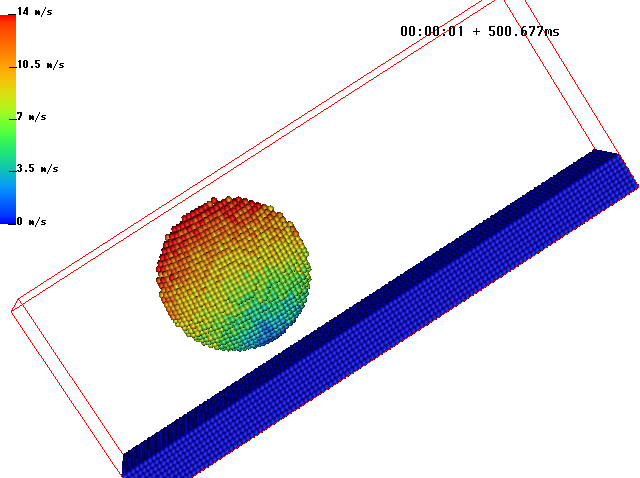
\includegraphics{inclinedPlaneSphere.png}}
  \caption{Sphere rolling down an ``inclined" plane.  The gravity vector
is oriented at a 45 degree angle relative to the plane.  Particles are colored
by velocity magnitude.}
  \label{figincplaneSphere}
\end{figure}

\bibliography{../references}

\end{document}
